\documentclass[12pt,letterpaper,oneside]{article}

% The file intend to keep track of good practices in Latex writing.

%==============================
% DOCUMENT
%==============================

% Fix some error reporting
\vfuzz2pt % Don't report over-full v-boxes if over-edge is small
\hfuzz2pt % Don't report over-full h-boxes if over-edge is small

% All the same, there are commands, classes and packages which are outdated and superseded. 
% nag provides routines to warn the user about the use of those.
\usepackage[l2tabu,orthodox]{nag}

%==============================
% BIBLIOGRAPHY
%==============================

% \addbibresource{references.bib} % in your preamble
% \citet{key}, \citep{key} % in the document
% \printbibliography % to generate the reference section
\usepackage[
backend=bibtex8,
style=ieee,
sorting=none,
natbib=true,
doi=false,
isbn=false,
url=false,
eprint=false,
maxcitenames=1,
mincitenames=1
]{biblatex}

\makeatletter
\newcommand{\tempmaxup}[1]{\def\blx@maxcitenames{99}#1}
\makeatother

\DeclareCiteCommand{\fullcite}[\tempmaxup]
{\usebibmacro{prenote}}
{\usedriver
	{}
	{\thefield{entrytype}}}
{\multicitedelim}
{\usebibmacro{postnote}}

%==============================
% TEXT
%==============================

% \autoref{key} % instead of Figure~\ref{key}, Table~\ref{key}, or Section~\ref{key}
\usepackage[pdftex,colorlinks]{hyperref}
\def\sectionautorefname{Section}
\def\subsectionautorefname{Section}

% \acrodef{ICP}{Iterative Closest Point} % in the preamble
% \ac{ICP} % in the document
\usepackage[printonlyused]{acronym}

% International unit system 
% e.g., \SI{1000}{\m\squared}, \num{20000}
\usepackage{siunitx}
\sisetup{group-separator = \text{\,}} % small space for thousand separator

% avoid single line on a page or single line under a figure
% no command to use
\usepackage[all]{nowidow}

%==============================
% FIGURE
%==============================

% Preferred figure format:
% - pdf or eps for graphs and schemas
% - jpg for photo

% \includegraphics[width=\textwidth]{filename}
\usepackage[pdftex]{graphicx}

% convert eps to pdf, you need to skip the file extension to work properly
% \includegraphics{filename} % instead of \includegraphics{filename.eps}
\usepackage{epstopdf}

% for Inkscape figures, import tex files in other folder and keep paths coherent
% e.g., \import{images}{timeline.pdf_tex}
\usepackage{import}

% include path for logos
\graphicspath{{./latexGoodPractices/}}

%==============================
% TABLE
%==============================

% Cleaner spacing for tables
% \toprule, \midrule, \bottomrule % instead of \hline
\usepackage{booktabs}

% Tables that can fit page length
% e.g.,three columns with the second one being twice as large as the others
% \begin{tabu}{X X[2] X}
\usepackage{tabu}

%==============================
% MATH
%==============================

% Better symboles
\usepackage{amssymb,amsfonts,amsmath,amscd}

% \bm % in equations for proper bold font
\usepackage{bm} 

% Some handy commands
\newcommand{\norm}[1]{\left\Vert#1\right\Vert}
\newcommand{\abs}[1]{\left\vert#1\right\vert}
\newcommand{\set}[1]{\left\{#1\right\}}
\newcommand{\Real}{\mathbb R}
\newcommand{\bbm}{\begin{bmatrix}}
\newcommand{\ebm}{\end{bmatrix}}




%==============================================================
% FILL THIS SECTION

%\newcommand{\projectTitle}{Optimisation de la trajectoire 3D au moyen de stations totales robotiques ou GNSS en vue de l'obtention d'une précision subcentimétrique pour l'amélioration de système de carthographie dynamique pour la robotique mobile} % Génération de la trajectoire 6D pour l'amélioration d'algorithme de cartographie pour les véhicules autonomes/robotique mobile
\newcommand{\projectTitle}{Improving the robustness of motion modelling and control for mobile robots in harsh conditions}
\newcommand{\runningTitle}{Improving the robustness of motion modelling and control for mobile robots in harsh conditions}
\newcommand{\projectStudent}{Dominic Baril}
\newcommand{\projectStudentNIP}{111 103 819}
\newcommand{\projectDate}{December 2023} 

\newcommand{\projectSupervisor}{Prof. F. Pomerleau}
\newcommand{\projectCoSupervisor}{Prof. P. Gigu\`{e}re}

\newcommand{\afaire}[1]{\textcolor{red}{#1}}

% Change to your specific bibliography file
%\addbibresource{./latexGoodPractices/exampleReferences.bib}
\addbibresource{./references.bib}
%==============================================================

% ---------------------------------------------------------------
% Load style
%----------------------------------------
% Page style

% Set the page size
\addtolength{\hoffset}{-1.0in} \addtolength{\voffset}{-0.75in}
\setlength{\textwidth}{7in} \setlength{\textheight}{8.25in}
\setlength{\headheight}{0.6in}
\setlength{\headsep}{0.2in}

\setlength{\footskip}{40pt}
\setlength{\fboxsep}{12pt}

% Set the paragraph skip
\setlength{\parskip}{3pt}

% Access to a counter for the number of pages
\usepackage{lastpage}

% To allow text justify on the right
\usepackage{ragged2e}

%language package
\usepackage[english,francais]{babel}
\usepackage[utf8]{inputenc}  
\usepackage[T1]{fontenc}


%----------------------------------------
% Title style

\newcommand{\makeCustomTitle}
{
\begin{center}
\LARGE{\textbf{\projectTitle{}}}
\\
\vspace{5pt}
\normalsize{\projectStudent{} (\projectStudentNIP{})}
\\
\projectDate{}
\end{center}
\begin{flushright}
\footnotesize{Supervisé par \projectSupervisor{} 
\\
et co-supervisé \projectCoSupervisor{}}
\end{flushright}
}

% Set the style for matrix and vector
\newcommand{\vect}[1]{\bm{#1}}
\newcommand{\mat}[1]{\bm{#1}}

%----------------------------------------
% Section style
\usepackage{sectsty}

% Set the section labeling font
\allsectionsfont{\textsf\bfseries}

%----------------------------------------
% Caption style
\usepackage[font=small, labelfont=bf, skip=5pt]{caption}

%----------------------------------------
% header style
\usepackage{fancyhdr}



% Define the title page style
\fancypagestyle{titlePage}{%
\fancyhf{}%

\fancyhead[L]{
\includegraphics[height=0.45in]{UL_N}}
\fancyhead[C]{\raisebox{0.2in}{\textsc{Proposition de Th\`{e}se de doctorat}}}
\fancyhead[R]{
\includegraphics[height=0.45in]{norlab_logo_acronym_dark}}
\fancyfoot[C]{\thepage/\pageref*{LastPage}}

\renewcommand{\headrulewidth}{0.1pt}
\renewcommand{\footrulewidth}{0.2pt}
}

% Define the page style for the other pages
\fancypagestyle{plain}{%
\fancyhf{}
\fancyhead[L]{\runningTitle{}}
\fancyfoot[C]{\thepage/\pageref*{LastPage}}
\renewcommand{\headrulewidth}{0.1pt}
\renewcommand{\footrulewidth}{0.1pt}
}

% Set the page style for all the document except the first page
\pagestyle{plain}

%----------------------------------------
% footnote style
\usepackage{fnpos}
% Fix the footnotes location
\makeFNbottom \makeFNbelow

% ---------------------------------------------------------------
% Author

\author{\projectStudent{} \\
       Laval University\\
       1065, av. de la Médecine \\
       Quebec, Qc \\
       Canada G1V 0A6 \\
}

% ---------------------------------------------------------------
% PDF setup
\hypersetup{%
    pdftitle={\projectTitle},
    pdfauthor={\@author},
    pdfkeywords={research, project, robotics, norlab, Northern Robotics Lab, PhD's},
    pdfsubject={},
    pdfstartview={},
    urlcolor=cyan,
    linkcolor=red,
}%

% produce Gantt Chart
\usepackage{pgfgantt}
% ---------------------------------------------------------------

% Colored text
%\usepackage[dvipsnames]{xcolor}

%\usepackage{subfig}
\usepackage{graphicx}

%\usepackage{ulem}

\usepackage{array, tabularx} % FP: lire le fichier latex good practice
\renewcommand{\arraystretch}{1.2} 

% Fill the template with text
\usepackage{lipsum}
\newcommand{\lightlipsum}[1][0]{\textcolor{gray!50}{\lipsum[#1]}}

% Customize enumerate list
\usepackage{enumerate}

\usepackage{lscape}
\usepackage{pdflscape}
\usepackage{sidecap}
\usepackage{subcaption,graphicx}

\usepackage{longtable}

\makeatletter
\renewcommand\paragraph{\@startsection{paragraph}{4}{20pt}%
            {-2.5ex\@plus -1ex \@minus -.25ex}%
            {1.25ex \@plus .25ex}%
            {\normalfont\normalsize\bfseries}}
            \makeatother
\setcounter{secnumdepth}{4} % how many sectioning levels to assign numbers to
\setcounter{tocdepth}{4}    % how many sectioning levels to show in ToC

% Acronyms
\acrodef{GNSS}{Global Navigation Satellite System}
\acrodef{ICP}{iterative closest point}
\acrodef{ROC}{radius of curvature}
\acrodef{UGV}{uncrewed ground vehicle}
\acrodef{SSMR}{skid-steering mobile robot}
\acrodef{DRIVE}{Data-driven Robot Input Vector Exploration}
\acrodef{GP}{Gaussian process}
\acrodef{BLR}{Bayesian linear regression}
\acrodef{WILN}[WILN]{Weather-Invariant Lidar-based Navigation}
\acrodef{CADC}{Canadian Adverse Driving Conditions}
\acrodef{GF}{Gyro-free}
\acrodef{INS}{Inertial Navigation System}
\acrodef{MPC}{Model Predictive Control}


%================================================================
\begin{document}
\makeCustomTitle
\thispagestyle{titlePage}


% ---------------------------------------------------------------
\section{Introduction}
\label{sec:introduction}

The field of mobile robotics has known significant advances in the last decade, leading to potentially disruptive innovations in automation for various industries.
Autonomous systems are currently mature enough to be functional in controlled and structured operational environments, such as warehouses and urban areas under ideal weather.
\acp{UGV} are proving to be effective solutions to current society issues related to labor shortage, workplace security and operational efficiency. 
However, such issues are greater for industries industries such as agriculture, forestry, defense, mining and search and rescue,  which require operation in outdoors, uncontrolled environments.
In these cases, systems are subject to a higher spectrum of environmental hazards, such as harsh weather, traction variability and deployment in remote environments.
However, as stated by~\citet{VanBrummelen2018}, challenges inherent to these conditions remain an open question.

This work aims to extend proficiency and robustness of autonomous navigation systems to off-road environments and harsh weather. 
Autonomous navigation can be split into three key components: path planning, path following and localization. 
This work mainly focuses on path following, with some contributions to localization.
For path following, the key problems arising from navigating in such environments are the high variability of wheel-to-ground traction and complex vehicle dynamics.
For localization, the key problems are related to navigating in~\ac{GNSS}-denied conditions, low geometrical constraints and dynamic environments.
In all, the research question for this work can be stated as follows:

\begin{center}
	\emph{
		How to increase robustness of~\ac{UGV} path following and localization for off-road and winter conditions?
	}
\end{center}

A~\ac{UGV} motion model is a key component to compute optimal commands with respect to motion predictions and provide localization prior for localization systems. %TODO CITATIONS
Thus, this research project is focused at minimizing motion prediction error for models, which is directly correlated with path following and localization errors. 
Current approaches for~\ac{UGV} modeling belong to two families: Model-based, divided between kinematic and dynamic models, and Learning-based, leveraging machine learning and driving data to predict motion.
Both kinematic models and learning-based approaches share the advantage that they have a low expertise requirement for deployment and require a training dataset to reduce prediction error, leading them being the most popular choice.
To answer the aforementioned research question, three key issues were identified:

\begin{enumerate}\bfseries
  	\item How does~\ac{UGV} behavior differ between concrete and snow-covered terrain navigating. What kinematic model behaves best for both?
  	\item How can we standardize training dataset gathering and improve vehicle slip learning?
	\item What are the impacts of the boreal forest environment and winter weather on lidar-based localization?
\end{enumerate}

These key issues guide the scientific contributions that were made through this work.
The reminder of this document describes the current scientific production done through this project and upcoming plan up to thesis submission.
More specifically,~\autoref{sec:submitted} describes the currently submitted and published research work, summarizing contributions and lessons learned for each paper. 
Afterwards,~\autoref{sec:recherches_futures} details the remaining research work~\autoref{sec:calendrier} and provides a schedule leading to thesis submission.
Lastly,~\autoref{sec:conclusion} provides a brief conclusion.

%\newpage

% ---------------------------------------------------------------
\section{Current scientific production}
\label{sec:submitted}

This section describes the current scientific done through this Ph.D. thesis work and collaborations done with other researchers. 
First, the three articles conducted directly for which I acted as first author.
All of these scientific contributions are related to the subproblems states in~\autoref{sec:introduction}.
Then all of the worth in which I have participated as co-author is described briefly.
Since mobile robotics is a field requiring various expertise and human ressources to conduct field deployments, all scientific production presented includes multiple co-authors.

%\subsection{Format de soumission des papiers avec co-auteurs}

%Le champ de la robotique mobile est un domaine qui exige une expertise dans plusieurs domaines.
%C'est pourquoi mes publications ont été faites en collaboration avec plusieurs co-auteurs œuvrant dans des domaines connexes.
%Typiquement, le premier auteur est la personne dirigeant les efforts et tâches à effectuer pour la publication du papier (i.e. typiquement un étudiant faisant de la recherche), tandis que les derniers co-auteurs sont ceux conseillant sur la stratégie de publications ainsi que sur la vision à long terme du projet (i.e. typiquement un professeur ou chercheur supervisant le travail de l'étudiant).
%Quant aux autres co-auteurs, ils aident à effectuer plusieurs parties du travail de recherches, que ce soit pour aider à faire les expériences sur le terrain, pour traiter les résultats, pour finaliser l'écriture de la théorie ou pour aider à la rédaction.
%Mon rôle en tant que premier auteur fut de définir la problématique que les papiers aborderont, de travailler sur la théorie et la partie expérimentale avec le traitement des données, et enfin la supervision de la rédaction du papier.

\subsection{Articles published and submitted as first author}
\begin{center}
	\textbf{\fullcite{Baril2020}}
\end{center}
The first article that I have published was submitted to the ``Conference on Robot and Vision (CRV)'', in May 2020.
This article aims to evaluate the performance of~\acp{SSMR} kinematic motion models on dry concrete and snow-covered terrain.
For this article
In this article, we collected a total of~\SI{2}{\kilo\meter} of human driving data to evaluate four kinematic models from the literature.
We leverage lidar point cloud registration based on the~\ac{ICP} algorithm to generate ground truth localization.
The resulting contributions are as follows:
\begin{enumerate}
	\item validate their fitness for a heavier platform on a relatively uniform concrete terrain;
	\item evaluate their performance for snow-covered terrain using more than \SI{2}{\kilo\meter} of trajectories traveled; and
	\item highlight the impact of angular motion on the accuracy of \acp{SSMR} kinematic modeling.
\end{enumerate}

The four kinematic models evaluated are the extended differential-drive asymmetrical, the extended differential-drive symmetrical~\citep{Mandow2007}, the full linear~\citep{Anousaki2004} and~\ac{ROC}-based~\citep{Wang2015}.
We also show that models with less parameters tend to perform better for angular prediction and models with more parameters perform better for translation prediction, due to their ability to predict non-zero lateral motion.
However, once trained, the performance of all models is similar for both terrain types, suggesting that all kinematic models evaluated behave similarly.
The largest prediction error occurs when the vehicle's angular velocity is at its maximum, which leads to the highest amount of vehicle slip.

Additionally, training kinematic models with empirical driving data leads to significant prediction error reduction, for both concrete and snow-covered terrain.
The relation between training window and prediction error is also studied in this work, clearly showing that models perform best when predicting for the same horizon for which they were trained.
We show that for the same commanded angular velocity, angular velocity is higher on snow-covered terrain than concrete. 
This phenomenon is due to the high friction caused by the tire deformation occurring during skidding on concrete, compared to soft terrain deformation on snow-covered terrain.

The take home message for this published paper was that kinematic motion models are adequate for predicting~\ac{SSMR} motion, both on dry concrete and snow-covered terrain, however they require a training dataset dependent to vehicle and terrain properties.
During the experimental work conducted for this paper, we imitated similar work by having a human operator to stimulate as many commands as possible, however this process lead to biased command stimulation and forward-only driving and proved to be time-consuming.
Since deploying~\acp{UGV} in off-road environments is a complex endeavor, reducing the time requiring to generate a motion model that is accurate enough for stable autonomous navigation is key.

\begin{center}
	\textbf{\fullcite{Baril2023}}
\end{center}

Le second article sur lequel j'ai travaillé a été soumis à la conférence appelée ``International Conference on Robotics and Automation (ICRA)'', en septembre 2023.
Cet article se concentre sur les différentes méthodes de calibration extrinsèque employées pour exprimer les données provenant de plusieurs stations totales robotiques dans un référentiel commun, et répond donc à la deuxième problématique de mes travaux de recherches.
Dans cet article, nous proposons une nouvelle méthode dynamique qui se base sur les trois prismes suivis par nos trois stations totales robotiques.
Une comparaison est effectuée entre toutes les méthodes étudiées: la nôtre augmente la précision de \SI{25}{\%} par rapport à la meilleure des méthodes utilisées dans l'état de l'art.
Pour cet article, j'ai rédigé une bonne partie du texte, développé une partie du code pour le traitement des données, fait les expériences sur le terrain, et interprété les résultats obtenus.
La citation complète de ma publication est la suivante:

L'article décrit dans un premier temps l'état de l'art à propos des différentes méthodes de calibration extrinsèque existantes en géomatique et arpentage.
La première méthode est appelée calibration en deux-points.
Elle a uniquement besoin de deux points statiques dont on connaît très précisément la position relative, au moins au millimètre près.
Les positions sont mesurées par chacune des stations totales et la méthode nous donne les transformations rigides ente les référentiels respectifs.
La seconde méthode, qui est la plus utilisée pour faire une calibration extrinsèque, est celle des points statiques de calibration.
Cette méthode consiste à prendre les positions statiques de nombreux points de contrôles, à recaler leurs positions, ce qui nous donne les transformations rigides entre les référentiels respectifs des stations totales.
La troisième méthode est identique à celle précédemment citée, mais la position des points de contrôle est prise de manière dynamique avec un prisme en mouvement. 
Toutes ces méthodes, en plus de la nouvelle que nous proposons, sont décrites mathématiquement dans la section théorie du papier.
L'état de l'art du papier donne également les principales sources de bruits à prendre en compte lors d'expérimentations avec plusieurs stations totales robotiques.

La nouvelle méthode de calibration extrinsèque que nous proposons se base sur les distances inter-prismes positionnées sur la plateforme robotique.
Les distances pouvant être déterminées au millimètre près avec une station totale, nous pouvons minimiser la distance de ces distances inter-prismes avec une fonction de coût optimisée dans l'algèbre de Lie par une méthode des moindres carrés. 
Le résultat de cette minimisation nous donne directement les transformations rigides entre les référentiels des différentes stations totales robotiques.
Pour pouvoir appliquer cette minimisation, nous pré-traitons les données brutes provenant des stations totales avec un pipeline dédié filtrant les données dans un premier temps. 
Puis, dans un deuxième temps, celles-ci sont interpolées permettant les mesures des stations totales à un même instant.
Ceci n'est pas le cas habituellement puisque les données sont prises de manière asynchrone.

Afin de comparer les différentes méthodes, un jeu de données totalisant plus de \SI{30}{km} de trajectoire de la plateforme robotique a pu être enregistré lors de 40 expériences différentes: elles ont été réalisées entre fin février 2022 et septembre 2022 lors de 15 déploiements.
Ces déploiements se déroulèrent dans deux types d'environnement: à l'extérieur, tout d'abord sur le \underline{campus de l'Université Laval} où se situent des bases de calibrations statiques permettant de réaliser la calibration en deux-points, puis dans les \underline{tunnels de l'Université Laval}, longs et droits sur plusieurs centaines de mètres à certains endroits.
Le choix s'est porté sur ces lieux du fait de leurs différentes configurations spatiales et des expériences de cartographie 3D avec lidars qu'y mène le Norlab.
Comme suite à chaque déploiement, une station totale a mesuré la position des prismes et de certains capteurs avec précision afin que notre nouvelle méthode de calibration extrinsèque puisse être appliquée.

Grâce à ce jeu de données, des tests de sensibilités et d'ablations ont pu être effectués sur les différents paramètres et modules du pipeline de pré-traitement.
Il a été démontré que le pipeline augmente la précision des résultats de \SI{18}{\%} grâce au filtrage des données erronées.
De plus, une simple interpolation linéaire des données est suffisante en comparaison d'une utilisation de ``Gaussian Process'' pour laquelle une meilleure précision était attendue.
La comparaison entre les différentes méthodes de calibration extrinsèque nous démontre que la nôtre est la plus précise.
Son exactitude est cependant plus faible de quelques millimètres en comparaison de la méthode des points de contrôles statiques.
Globalement, toutes les méthodes sont plus précises que l'utilisation de \ac{GNSS}.

Dans cet article, nous avons proposé une nouvelle méthode de calibration extrinsèque qui ne se base pas sur la mesure de points statiques, ce qui permet d'augmenter le temps consacré aux expériences lors de déploiements.
Cette nouvelle méthode s'accompagne d'un pipeline de pré-traitement des données venant des stations totales robotiques. 
L'utilisation du pipeline augmente de \SI{18}{\%} la précision des résultats, et ceux-ci sont plus précis de \SI{25}{\%} car combinés à notre nouvelle méthode de calibration extrinsèque.
Notre nouvelle méthode de calibration est limitée dans certains types d'environnements comme les tunnels, où les trajectoires sont longues et droites, ce qui empêche notre minimisation de converger vers le résultat attendu.
Des simulations plus poussées seront effectuées afin de mieux caractériser ces limites d'utilisation.
La position des prismes sur la plateforme robotique a également un effet sur le résultat, qui doit être davantage quantifié avec précision. 
Cet article met à notre disposition tous les moyens de recueillir des données précises permettant de reconstruire les vérités terrains précises qui seront utiles pour l'évaluation des algorithmes de cartographie 3D.
Le code ainsi que le jeu de données utilisés sont disponibles en ligne \footnote{\url{https://github.com/norlab-ulaval/RTS_Extrinsic_Calibration}}.

\subsection{Articles published and submitted as co-author}

\textbf{\fullcite{Vlad2022}}: 
Ce papier présente un moyen d'améliorer la précision de la localisation par lidar grâce à la prise en compte du vecteur de gravité donné par une centrale inertielle. 
Pour ce papier, j'ai effectué les comparaisons de trajectoire entre celles données par notre algorithme de cartographie amélioré et celles des vérités terrains prises par des \ac{GNSS}. 
J'ai également apporté mon aide à la prise de jeux de données sur le terrain et à la rédaction.
\\

\textbf{\fullcite{Baril2022}}:
Cet article de journal présente un pipeline de ``teach-and-repeat'' qui a été testé en forêt Montmorency. 
Avec ce pipeline, la plateforme robotique a pu effectuer près de \SI{20}{km} de trajectoire en toute autonomie, dans des conditions boréales. 
Pour ce faire, j'ai enregistré sur le terrain des données de vérités terrains à l'aide de mon système de stations totales et de \ac{GNSS}, puis j'ai traité les données recueillies. 
J'ai également participé à la rédaction de l'article.
\\

\textbf{\fullcite{Roucek2021}}:
En février 2020, j'ai participé à la compétition du DARPA (``Defense Advanced Research Projects Agency'') Urban Challenge. 
Ce papier présente le système utilisé lors de la compétition, ainsi que les résultats obtenus. 
J'ai participé à la compétition, traité les données en lien avec la cartographie 3D et effectué l'évaluation de la précision de notre algorithme pour la localisation des plateformes utilisées.
\\

\textbf{\fullcite{Chahine2021}}: 
Ce papier présente un algorithme de cartographie 3D se basant sur différents capteurs visant ainsi à améliorer la précision du résultat (lidar, caméra et \ac{GNSS} ensemble).

C'est dans ce papier que j'ai présenté pour la première fois le début de mes recherches avec mon système de stations totales. 
Mais seule une station totale a pu alors être utilisée du fait du manque d'espace pour les cibles sur le sac à dos avec les capteurs.
J'ai aidé à la prise de données sur le terrain, ainsi qu'à leur traitement pour l'obtention de la vérité terrain, et j'ai également participé à la rédaction de l'article.
\\

\textbf{\fullcite{Baril2020}}:
Cet article présente l'évaluation de modèle cinématique sur différents types de terrains: asphalte ou neige. 
Le but de l'article est de présenter les résultats des différents modèles et de discuter de leur efficacité. 
Pour cet article, j'ai pris des données sur le terrain et j'ai traité celles provenant de notre algorithme de cartographie. 
J'ai également aidé à la rédaction.
\\

\textbf{\fullcite{Laconte2021}}:
Ce papier présente l'état de l'art pour les différentes méthodes de localisation de véhicules sur des autoroutes, principalement par la détection des lignes via des systèmes de caméras et de lidars.
J'ai aidé à la rédaction de l'article. Aucune donnée n'a été prise sur le terrain.
\\

\textbf{\fullcite{Vaidis2020}}:
Cet article est un article de ``workshop'' pour la conférence ICRA 2021, en ce sens non pertinent pour ma thèse.
Il aborde l'amélioration de notre algorithme de cartographie avec des contraintes de rotation fixées dans l'algèbre de Lie via des données issues d'une centrale inertielle.
Pour ce papier, j'ai effectué les expériences, traité les données et rédigé la grande partie de l'article.
%\newpage

% ---------------------------------------------------------------
% \section{Expériences/déploiements réalisés}
\label{sec:experiences_faites}

\begin{figure}[!t]
    \centering
    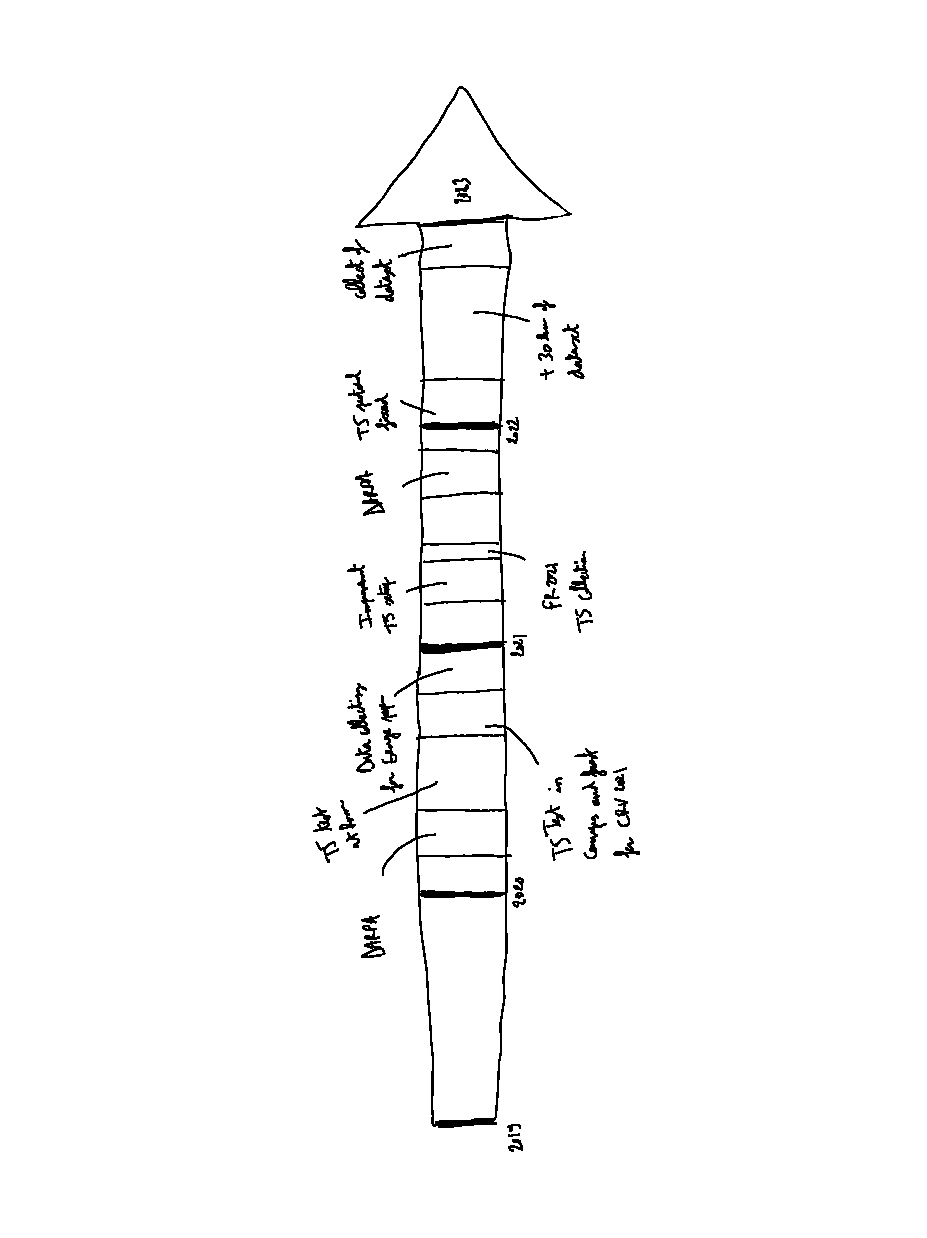
\includegraphics[width=\linewidth, angle=0, trim={0 0 0 0},clip]{figs/TS_timeline.pdf}
    \caption{Ligne de temps travaux TS}
    \label{fig:frise_exp}
\end{figure}

Au cours des quatre premières années de mon doctorat, j'ai effectué beaucoup de déploiements sur le terrain afin de tester et valider mes protocoles de déploiements, que ce soit pour mes stations totales robotiques, ou pour les plateformes robotiques que l'on utilise.
Cette section est destinée à détailler davantage les déploiements  illustrés sur la frise chronologique \autoref{fig:frise_exp}.
Les déploiements principaux ont été faits pour tester le système de stations totales dans différents types d'environnements.
Vient ensuite le DARPA challenge avec le déploiement de plateforme robotique dans des environnements souterrains.
Enfin, quelques déploiements annexes à mes recherches ont été réalisés en lien avec la prise de vérités terrains pour comparer des algorithmes de cartographie ou de contrôle.

\subsection{Stations totales robotiques}

La très grande majorité des déploiements avait pour but de  développer le système de stations totales robotiques.
Ces dernières ont été reçues au début de l'hiver 2020 et j'ai concrétisé le développement du code permettant de les faire fonctionner au printemps 2020.
Le système de collecte des données fut tout d'abord testé correctement en laboratoire,puis en environnement extérieur,sur le campus de l'université et en forêt de Montmorency, durant l'été et l'automne 2020.
Les données alors recueillies ont permis de rédiger le papier de CRV 2021.

À la suite de la publication de CRV 2021, de nouveau tests sur le campus et en forêt ont été réalisés au printemps 2021 afin d'améliorer le système d'acquisition des données. 
Le protocole de déploiement du système a été travaillé et finalisé entre octobre 2021 et février 2022 à la suite d'une bonne douzaine de déploiements.
Il se résume ainsi : si on utilise le système des stations totales pour un déploiement, on est sûr à 100\% d'avoir nos données, ce qui n'était pas le cas précédemment du fait de problèmes techniques ou d'une mauvaise utilisation des équipements.
 Trois expériences consécutives réussies sans problème pour l'acquisition des données ont validé le protocole.

 Le protocole stabilisé a permis la collecte du dataset pour le papier d'ICRA 2023 ( fin février 2022 jusqu'à mi-septembre 2022).
Cette collecte a été faite dans deux types d'environnements principaux, à savoir sur le campus de l'Université Laval en extérieur, mais aussi dans ses tunnels.
L'extérieur a été utilisé afin de pouvoir récolter des données \ac{GNSS} et de les comparer avec le système de stations totales.Mais là, il fut également possible d'accéder à des pylônes de calibration utilisée en géomatique, au positionnement relatif connu au millimètre près.La comparaison entre différentes méthodes de calibration extrinsèque fut ainsi aussi rendue possible.
Les tunnels ont été utilisés puisque des expériences de cartographie ont été menées pour un projet annexe de fin de maîtrise, et que, dans ce cas, des vérités terrains se révélaient nécessaires.
Deux plateformes robotiques ont été déployées, à savoir un Warthog de la compagnie ClearPath, et un HD2 de la compagnie SuperDroid.
Au total, le dataset se compose de 15 déploiements constitUtifs de 40 expériences,lesquelles totalisent plus de 32 kilomètres de trajectoires des plateformes robotiques.
Ce dataset est disponible en ligne. \href{https://github.com/norlab-ulaval/RTS_Extrinsic_Calibration/wiki/RTS-2022-Dataset}{ici}.

\subsection{DARPA}

Description DARPA competition, pourquoi relié à mes recherches

DARPA URBAN

DARPA FINALS

\subsection{Projets annexes en lien avec stations totales robotiques}

Projets annexes utilisant les stations totales, condition utilisation et pourquoi (amélioration algorithme)

Georges project

FR 2021 - teach-repeat

Matej project

% ---------------------------------------------------------------
\section{Recherches futures}
\label{sec:recherches_futures}

Dans les \autoref{sec:papiers_soumis} ont été présentés le travail réalisé pour mettre au point le système de stations totales robotiques, ainsi que la collecte de données dans différents types d'environnement avec une précision sub-centimétrique.
Les deux premières problématiques de mon doctorat concernant la mise au point de ce système de collecte de données ainsi que l'obtention d'une calibration extrinsèque de précision ont été détaillées et résolues.
La présente section détaille les travaux de recherches que je planifie afin de répondre à ma dernière problématique de recherche, à savoir comment utiliser les données récoltées pour générer des vérités terrains précises dans l'ordre du millimètre, et effectuer des comparaisons de trajectoires avec ces vérités terrains.
Le calendrier détaillé de mes recherches restantes est présenté dans la \autoref{sec:calendrier}.

\subsection{Génération de vérités terrains}

La dernière partie de mon doctorat se concentrera donc sur la génération des vérités terrains, ce qui est la suite logique de mes travaux de recherches, ainsi que le but ultime de mon système de stations totales robotiques.
Cette dernière problématique se décompose en trois sous-parties:

\begin{enumerate}\bfseries
    \item La génération des vérités terrains,
    \item La gestion de l'incertitude,
    \item L'évaluation de trajectoires avec ces vérités terrains.
\end{enumerate}

La génération de vérités terrains, à savoir la pose de la plateforme robotique en six degrés de liberté, a déjà été succinctement évoquée dans le papier CRV 2021: sa faisabilité a été démontrée.
Celle-ci a été effectuée après l'interpolation des trajectoires de prismes par une minimisation point-à-point entre les positions théoriques des prismes les uns par rapport aux autres, et leurs positions mesurées sur le terrain.
Dans le papier d'ICRA 2023, nous avons relaté que l'utilisation de modules de filtrage permettait d'augmenter la précision de \SI{18}{\%} des résultats finaux.
Nous souhaitons appliquer le même principe à la génération des vérités terrains pour en augmenter la précision, et utiliser d'autres méthodes d'interpolation ou d'optimisation de trajectoires pour générer ces vérités terrains et évaluer quelles en sont les meilleures, notamment pour quantifier l'incertitude.

L'incertitude est rarement quantifiée lors de la génération de vérités terrains.
Elle l'est encore moins pour l'évaluation de trajectoires par rapport à celles-ci.
Avec notre système de trois stations totales et des trois prismes, nous avons la possibilité de pouvoir estimer l'incertitude grâce à la métrique de la distance inter-prisme.
C'est pourquoi l'objectif de mes prochaines recherches portera sur la manière de quantifier cette incertitude à l'aide des expériences effectuées.
Mon souhait est également d'exploiter cette incertitude pour ce qui concerne la comparaison de trajectoires.

L'évaluation de trajectoires avec des vérités terrains se fait depuis de nombreuses années.
La très grande majorité des évaluations utilise la norme euclidienne pour établir les comparaisons.
Cette norme est facile à mettre en application, mais elle ne prend pas en compte l'incertitude, ce qui peut fausser le résultat et donc rendre inutilisable la vérité terrain.
Ces situations peuvent se produire lorsqu'un \ac{GNSS} est utilisé pour générer une vérité terrain, alors que son signal n'est pas bon.
Une incertitude de plusieurs mètres peut alors apparaître comme ce fut le cas pour le jeu de données du Kitty Dataset \footnote{\url{https://www.cvlibs.net/datasets/kitti/eval_odometry.php}}, lequel compare des trajectoires données par des algorithmes de cartographie à sa vérité terrain issue d'un \ac{GNSS}.
En dessous de \SI{100}{m} d'évaluation par une métrique d'erreur de pose relative, les résultats peuvent être biaisés.
Les auteurs du jeu de données ont donc mis la distance d'évaluation pour une métrique d'erreur de pose relative à \SI{100}{m} au minimum pour éviter ces cas.
Dans mes recherches, je souhaite améliorer la prise en compte de l'incertitude concernant l'évaluation de trajectoires.
Cela permettra un résultat plus représentatif pour effectuer des comparaisons d'algorithmes entre eux.

Ces trois sous-parties de ma problématique finale seront développées dans un article de journal que je soumettrai fin mars 2023.
Le journal visé sera celui de ``Field Robotics'' \footnote{\url{https://www.journalfieldrobotics.org/Field_Robotics/Home.html}}.
Cet article de journal se concentrera sur la manière dont on générera les vérités terrains avec notre système de stations totales robotiques.
Il sera une suite logique des deux premiers articles, et présentera des jeux de données provenant de déploiements effectués durant une année entière (février 2022 à décembre 2022) afin de pouvoir montrer la plus-value de notre système dans différents types d'environnements et dans différentes conditions météorologiques.
Le détail des expériences à faire est présenté dans la prochaine sous-section.

\subsection{Expériences prévues}

Afin de préparer mes recherches futures, plus d'une dizaine de déploiements sont prévus en ces mois de novembre et décembre 2022.
Je collecterai les données manquantes à la présentation de mon travail dans l'article de journal.
Ces déploiements sont répartis en plusieurs étapes correspondant à différentes parties de ma recherche, à savoir l'évaluation de la précision du système de stations totales robotiques dans différentes conditions, la comparaison de celle-ci avec les \ac{GNSS} sur un plus grand nombre de données, et la récolte de plus de données en forêt de Montmorency.

Quelques évaluations ont déjà été réalisées et répertoriées dans l'article de CRV 2021 sur notre système afin de caractériser la précision de ce dernier.
Cependant, le jeu de données alors utilisé comprenait moins de \SI{500}{m} de trajectoires de la plateforme robotique et la méthode de calibration extrinsèque utilisée n'était pas aussi précise que celle développée dans l'article d'ICRA 2023.
Quelques expériences pour mieux comprendre notre système font défaut au jeu de données utilisé dans l'article d'ICRA 2023: à savoir la distance limite de la prise de données due à la distance maximale permise par les stations totales ainsi que la distance maximale des modules LoRa de communication.
Des expériences seront donc menées afin de quantifier ces limites, mais également afin de quantifier la précision en fonction de la distance de la prise de mesure. 
De plus, dans les articles de CRV 2021 et d'ICRA 2023 a été soulevée la question de l'influence de la position des prismes sur la plateforme robotique.
Des simulations et des expériences seront menées afin de pouvoir répondre à cette question.

Dans l'article de CRV 2021, a été effectuée une comparaison avec des données \ac{GNSS} en milieux ouverts ainsi qu'en forêt.
Pour faire suite aux récentes améliorations apportées à notre système, une collecte de données plus conséquente sera réalisée dans le but d'augmenter le nombre de données exploitables en plus de celles utilisées pour le papier d'ICRA 2023. 
Les données \ac{GNSS} ont pour le moment uniquement servi à comparer la précision du système par rapport à la métrique de la distance inter-prisme ou inter-\ac{GNSS}.
Les données que nous récolterons prochainement serviront cette fois à faire des comparaisons de trajectoires avec les vérités terrains.
De plus, les trajets effectués prendront en compte différents types de scénarios, tels que l'alternance de milieux ouverts ou couverts, afin de mettre en évidences les problèmes des \ac{GNSS} comparés à notre système de stations totales.

Enfin, il est prévu de faire des déploiements en forêt de Montmorency dans le but de recueillir des données avec météo variable: par temps de brouillard et de chutes de neige afin de quantifier la précision de notre système pendant ces épisodes climatiques.
De ce fait, au moins deux déploiements sont prévus à un mois d'écart: le premier au début du mois de novembre 2022 (sans neige), puis le second au début du mois de décembre (avec neige).
Les deux plateformes robotiques seront utilisées afin de maximiser la prise de données durant ces déploiements.
Ces expériences visant à comparer les jeux de données seront cependant toujours réalisées au même endroit, quelle que soit la météo.

Il est à noter que pour chacun des déploiements effectués, les données provenant de capteurs lidars seront également récoltées afin de pouvoir comparer la trajectoire donnée par notre algorithme de cartographie 3D à celle issue de notre système de stations totales robotiques ou de \ac{GNSS}.
Ainsi, grâce à chaque expérience menée, nous pourrons étudier un résultat spécifique et le présenter dans l'article de journal.
Le jeu de données de l'article d'ICRA 2023 sera également exploité pour certains résultats et certaines comparaisons, comme cela avait été prévu initialement.
Au total, nous souhaitons avoir plus de \SI{50}{km} de trajectoires de plateforme robotiques afin d'éliminer certaines valeurs aberrantes lors de la génération des résultats, et pouvoir ainsi accéder à un jeu de données complet prenant en compte différents types d'événements.
Cela nous est nécessaire si nous souhaitons trouver les limites de notre système, comme ce fus le cas par exemple dans l'article d'ICRA 2023.
%\newpage

% ---------------------------------------------------------------
% \section{Calendrier administratif}
\label{sec:calendrier_admin}

Mon article de journal rédigé, je me concentrerai sur la rédaction de ma thèse.
La \autoref{fig:gantt} montre le calendrier de la planification des objectifs pour le dépôt final de la thèse.
Je souhaite réaliser une thèse par articles.
Elle en comportera trois que j'ai publiés ou soumis: CRV 2021, ICRA 2023 et Field Robotics 2023.
S'il est accepté, l'article d'ICRA 2023 sera présenté à la conférence à la fin du mois de mai 2023.
Pour ce qui est de l'article du journal Field Robotics, il sera probablement publié d'ici un an ou deux, soit en 2024 ou 2025, après les différentes rondes de révisions.

Je prévois deux mois de rédaction de thèse juste après la soumission de mon article de journal, soit en avril et mai 2023. 
Je ferai mon dépôt initial au mois de mai 2023.
Après une période de 6 à 8 semaines, je pourrai effectuer ma défense durant le mois de juillet 2023.
Si ma thèse est acceptée, il m'appartiendra de faire les corrections données par mon comité pour un dépôt final escompté au mois d'août 2023.

\setlength{\fboxsep}{9pt}
\begin{figure}[htbp]
  \centering
  \definecolor{navyblue}{RGB}{21,80,130}
\setganttlinklabel{f-s}{}

\begin{ganttchart}[
     %Specs 0.43 0.43 1
     y unit title=0.43cm,
     y unit chart=0.55cm,
     x unit=1.1cm,  %1.2cm
     vgrid={*{1}{draw=none},*{1}{black}},
     title height=1,   %1
     title label font=\bfseries\footnotesize,
     % bar 0.4 10pts
     bar/.style={fill=navyblue},
     bar height=0.4,
     bar label font=\footnotesize,
     bar label node/.append style={left=10pt},  %10
     % group 0 0.6 0.3 0.2 0.3 10pts
     group right shift=0,
     group top shift=0.6,
     group height=.3,
     group peaks width={0.2},
     group peaks height={0.3},
     group label node/.append style={left=10pt},
     group label font=\bfseries\footnotesize,
     % milestone 0.4 1 10pts
     milestone/.append style={xscale=0.4, yscale=1},
     milestone label node/.append style={left=10pt},
     milestone label font=\itshape\footnotesize
     ]{1}{8}
    \gantttitle[]{2024}{8}
    \\              
    \gantttitle{J}{1} \gantttitle{F}{1} \gantttitle{M}{1} 
    \gantttitle{A}{1} \gantttitle{M}{1} \gantttitle{J}{1} 
    \gantttitle{J}{1} \gantttitle{A}{1} 
    \\
    %--------------------------------------       
    \ganttgroup{Thesis writing}{1}{3}\\
    
    \ganttbar{Articles insertion}{1}{1}
    \ganttbar[inline, bar label font/.append=\color{white}]{}{1}{1}\\
    
    \ganttbar{Final results chapter}{2}{2}
    \ganttbar[inline, bar label font/.append=\color{white}]{}{2}{2}\\
    
    \ganttbar{Introduction, conclusion}{3}{3}
    \ganttbar[inline, bar label font/.append=\color{white}]{}{3}{3}\\
	
	\ganttmilestone{Thesis submitted}{3}\\
	
    %--------------------------------------       
    \ganttgroup{Final experiments}{1}{2} \\ 
    
    \ganttbar{DRIVE impact on UGV path following}{1}{2}
    \ganttbar[inline, bar label font/.append=\color{white}]{}{1}{2}\\
    
    %--------------------------------------       
    \ganttgroup{\emph{ICRA 2024}}{2}{5} \\ 
    
    \ganttbar{Paper corrections}{2}{2}
    \ganttbar[inline, bar label font/.append=\color{white}]{}{2}{2}\\
    
    \ganttmilestone{Re-submission}{2}\\
    
    \ganttbar{Presentation preparation}{5}{5}
    \ganttbar[inline, bar label font/.append=\color{white}]{}{5}{5}\\
    
    \ganttmilestone{Article presentation}{5}\\
    
    %--------------------------------------       
    \ganttgroup{Thesis defense}{4}{8}\\
    
    \ganttbar{Thesis review}{4}{6}
    \ganttbar[inline, bar label font/.append=\color{white}]{}{4}{6}\\
    
    \ganttbar{Defense preparation}{4}{6}
    \ganttbar[inline, bar label font/.append=\color{white}]{}{4}{6}\\
    
    \ganttmilestone{Defense}{6}\\
    
    \ganttbar{Final reviews}{7}{8}
    \ganttbar[inline, bar label font/.append=\color{white}]{}{7}{8}\\
    
    \ganttmilestone{Final submission}{8}\\
    
\end{ganttchart}

  \caption{Diagramme de Gantt contenant les objectifs devant être accompli d'ici au dépôt final de la thèse.
  }
  \label{fig:gantt}
\end{figure}
\setlength{\fboxsep}{12pt}
% \newpage

% ---------------------------------------------------------------
\section{Conclusion}
\label{sec:conclusion}

À travers cette proposition de thèse, un récapitulatif de mes contributions vis-à-vis de ma problématique de recherche a été présenté, et la planification de la fin de mon doctorat a été détaillée.
J'ai démontré que j'avais suffisamment avancé dans mes recherches et que je serai sur le point d'effectuer mon dépôt initial d'ici à quelques mois.
La problématique de ma recherche porte sur la génération précise de trajectoires de références pour les véhicules en mouvement ainsi que de leur évaluation.
Deux sous-parties de ma problématique de recherche ont déjà été abordés et résolus à travers la publication de deux articles de conférence, dont un soumis en septembre dernier.
Dans un premier temps, un système basé sur trois stations totales robotiques a été créé et testé sur le terrain dans le but de pouvoir générer des vérités terrains ayant une précision sub-centimétrique.
Par la suite, une amélioration de la calibration extrinsèque entre les différents référentiels de ces stations totales robotiques a été proposée et validée sur un jeu de données de plus de \SI{30}{km} de trajectoires de plateformes robotiques.
Mes travaux actuels portent sur la publication d'un dernier article de journal qui finalisera mes recherches.
Cet article abordera la problématique de l'évaluation des trajectoires de références accompagnée de celles générées par des algorithmes de cartographie 3D.
Il abordera également la gestion de l'incertitude dans ces évaluations et mentionnera l'impact de cette incertitude sur les résultats.

Le calendrier des étapes restantes a été détaillé dans la \autoref{sec:calendrier}.
La rédaction de mon article de journal aura lieu du mois de novembre 2022 au mois de mars 2023.
Ensuite sera effectuée la rédaction de ma thèse.
Je prévois une rédaction de thèse par articles comme cités dans ce document, à savoir l'article de CRV 2021, l'article de ICRA 2023 et l'article de journal Field Robotics 2023 que je rédigerai.
Le dépôt initial de ma thèse aura lieu au mois de mai 2023 et ma défense devrait se tenir durant le mois de juillet 2023.
Je prévois ainsi de terminer mon dépôt final durant le mois d'août 2023 après avoir effectué les corrections demandées suite à ma défense.


%\newpage
% ---------------------------------------------------------------
\printbibliography
%\newpage

% ---------------------------------------------------------------
%\begin{landscape}
%\section{Annexe}
\label{sec:Annexe}

\setlength{\fboxsep}{9pt}
\begin{figure}[htbp]
  \centering
  \definecolor{navyblue}{RGB}{21,80,130}
\setganttlinklabel{f-s}{}

\begin{ganttchart}[
     %Specs 0.43 0.43 1
     y unit title=0.43cm,
     y unit chart=0.37cm,
     x unit=0.7cm,  %1.2cm
     vgrid={*{3}{draw=none},*{1}{black}},
     title height=1,   %1
     title label font=\bfseries\footnotesize,
     % bar 0.4 10pts
     bar/.style={fill=navyblue},
     bar height=0.4,
     bar label font=\footnotesize,
     bar label node/.append style={left=10pt},  %10
     % group 0 0.6 0.3 0.2 0.3 10pts
     group right shift=0,
     group top shift=0.6,
     group height=.3,
     group peaks width={0.2},
     group peaks height={0.3},
     group label node/.append style={left=10pt},
     group label font=\bfseries\footnotesize,
     % milestone 0.4 1 10pts
     milestone/.append style={xscale=0.4, yscale=1},
     milestone label node/.append style={left=10pt},
     milestone label font=\itshape\footnotesize
     ]{1}{20}
    \gantttitle[]{2022}{8}
    \gantttitle[]{2023}{12}
    \\              
    \gantttitle{N1}{1} \gantttitle{N2}{1} \gantttitle{N3}{1} \gantttitle{N4}{1} \gantttitle{D1}{1} \gantttitle{D2}{1} \gantttitle{D3}{1} \gantttitle{D4}{1} \gantttitle{J1}{1} \gantttitle{J2}{1} \gantttitle{J3}{1} \gantttitle{J4}{1}
    \gantttitle{F1}{1} \gantttitle{F2}{1} \gantttitle{F3}{1} \gantttitle{F4}{1} \gantttitle{M1}{1} \gantttitle{M2}{1} \gantttitle{M3}{1} \gantttitle{M4}{1}
    \\
    %--------------------------------------       
    \ganttgroup{Déploiements et expériences}{1}{6}\\
    
    \ganttbar{Performances système}{1}{1}
    \ganttbar[inline, bar label font/.append=\color{white}]{}{1}{1}\\
    
    \ganttbar{Tests positions prismes}{2}{2}
    \ganttbar[inline, bar label font/.append=\color{white}]{}{2}{2}\\
    
    \ganttbar{Comparaison GNSS}{2}{5}
    \ganttbar[inline, bar label font/.append=\color{white}]{}{2}{5}\\
    
    \ganttbar{Déploiement forêt 1}{2}{2}
    \ganttbar[inline, bar label font/.append=\color{white}]{}{2}{2}\\
    
    \ganttbar{Déploiement forêt 2}{5}{5}
    \ganttbar[inline, bar label font/.append=\color{white}]{}{5}{5}\\
	
	\ganttmilestone{Ensemble des données récoltées}{6}\\
	
    %--------------------------------------       
    \ganttgroup{Reconstruction des trajectoires}{1}{8} \\ 
    
    \ganttbar{État de l'art}{1}{2}
    \ganttbar[inline, bar label font/.append=\color{white}]{}{1}{2}\\
    
    \ganttbar{Génération vérités terrains}{1}{4}
    \ganttbar[inline, bar label font/.append=\color{white}]{}{1}{4}\\
    
    \ganttbar{Tests méthodes interpolations}{1}{8}
    \ganttbar[inline, bar label font/.append=\color{white}]{}{1}{8}\\
    
    \ganttmilestone{Pipeline de génération fini}{8}\\
    
     %--------------------------------------       
    \ganttgroup{Utilisation de l'incertitude}{1}{12} \\ 
    
    \ganttbar{Impact positions des prismes}{1}{2}
    \ganttbar[inline, bar label font/.append=\color{white}]{}{1}{2}\\
    
    \ganttbar{Interpolation données brutes}{6}{8}
    \ganttbar[inline, bar label font/.append=\color{white}]{}{6}{8}\\
    
    \ganttbar{Obtention de l'incertitude}{8}{12}
    \ganttbar[inline, bar label font/.append=\color{white}]{}{8}{12}\\
    
    \ganttmilestone{Incertitude peut être évaluée}{12}\\
    
    %--------------------------------------       
    \ganttgroup{Évaluation de trajectoires}{3}{16} \\ 
    
    \ganttbar{Comparaison lidar-GNSS}{3}{5}
    \ganttbar[inline, bar label font/.append=\color{white}]{}{3}{5}\\
    
    \ganttbar{Comparaison des normes}{5}{8}
    \ganttbar[inline, bar label font/.append=\color{white}]{}{5}{8}\\
    
    \ganttbar{Usage de l'incertitude}{8}{12}
    \ganttbar[inline, bar label font/.append=\color{white}]{}{8}{12}\\
    
    \ganttbar{Niveau de précision}{12}{16}
    \ganttbar[inline, bar label font/.append=\color{white}]{}{12}{16}\\
    
    \ganttmilestone{Pipeline d'évaluation complété}{16}\\
    
    %--------------------------------------       
    \ganttgroup{Rédaction du journal}{1}{19} \\ 
    
    \ganttbar{Rédaction état de l'art}{1}{6}
    \ganttbar[inline, bar label font/.append=\color{white}]{}{1}{6}\\
    
    \ganttbar{Rédaction théorie}{3}{16}
    \ganttbar[inline, bar label font/.append=\color{white}]{}{4}{16}\\
    
    \ganttbar{Rédaction expériences}{6}{10}
    \ganttbar[inline, bar label font/.append=\color{white}]{}{6}{10}\\
    
    \ganttbar{Rédaction résultats}{10}{19}
    \ganttbar[inline, bar label font/.append=\color{white}]{}{10}{19}\\
    
    \ganttmilestone{Soumission du papier}{19}\\
    
\end{ganttchart}

  \caption{Diagramme de Gantt contenant les objectifs de recherche devant être accomplis d'ici au dépôt initial de la thèse pour la soumission de l'article de journal.
  }
  \label{fig:gantt_recherche}
\end{figure}
\setlength{\fboxsep}{12pt}
%\end{landscape}
%\newpage

\end{document}

